\chapter{Électronique} \label{electronique}
\section{Microcontrôleur}

\subsection{Introduction}

\subsection{Microprocesseur (\textit{µP})}
Un \textbf{microprocesseur} (\textit{µP}) est une 
\textbf{unité centrale de traitement} (\textbf{CPU}\footnote{Glossaire : \gls{cpu}}) qui exécute des 
instructions, mais qui \textbf{ne contient ni mémoire RAM, ni mémoire ROM, ni 
entrées/sorties intégrées}. Il est conçu pour des systèmes où ces composants, 
tels que la \textit{RAM}, la \textit{ROM}, et les \textit{interfaces}, sont 
ajoutés séparément sur une carte mère. Le \textit{microprocesseur} est 
principalement utilisé dans les \textbf{ordinateurs}, \textbf{serveurs}, et 
\textbf{systèmes embarqués avancés}, comme les processeurs Intel, AMD, ou Apple 
Silicon.\par

\subsection{Microcontrôleur (\textit{MCU})}
Un \textbf{microcontrôleur} (\textit{MCU}) est un \textbf{circuit intégré complet} 
qui inclut non seulement un \textbf{microprocesseur}, mais aussi de la 
\textbf{mémoire RAM}, de la \textbf{mémoire ROM (Flash)} et des 
\textbf{périphériques d'entrées/sorties} sur une seule puce. Cela lui confère un 
\textbf{plus haut degré d'intégration} par rapport à un microprocesseur. Il est 
également appelé un \textbf{Système sur une Puce} (\textbf{SoC}, 
\textit{System On a Chip}). Il est conçu pour exécuter des 
\textbf{tâches spécifiques} à un \textbf{coût réduit} et avec une 
\textbf{consommation d'énergie optimisée}. On le retrouve dans des 
\textbf{systèmes embarqués}, notamment dans des 
\textbf{appareils électroménagers}, des \textbf{voitures}, des 
\textbf{jouets électroniques}, et des \textbf{objets connectés}, comme les 
dispositifs basés sur \textit{Arduino}, \textit{STM32}, \textit{PIC}, et 
\textit{ESP32}.\par

\section{Le microcontrôleur ESP32}

Le microcontrôleur utilisé dans la mineure \textbf{Instrumentation} est 
l'\textbf{ESP32}, fabriqué par \textbf{Espressif Systems} (\textit{Chine}).

\subsection{Caractéristiques principales de l'ESP32}
Le \textbf{processeur} de l'ESP32 est un \textit{Dual-Core Xtensa LX6} qui peut 
fonctionner jusqu'à \SI{240}{\mega\hertz}, conçu par \textbf{Tensilica}. Il
dispose également d' \textbf{instructions DSP} (\textit{Digital Signal Processing}) 
intégrées, permettant le \textbf{traitement de signaux complexes}. En termes de 
\textbf{connectivité}, l'ESP32 supporte le \textbf{Wi-Fi}, le \textbf{Bluetooth}, 
ainsi que le \textbf{Bluetooth Low Energy (BLE)}. Il dispose également de 
\textbf{modes basse consommation}, ce qui est crucial pour les applications à 
faible consommation énergétique. Parmi les \textbf{interfaces de périphériques} 
disponibles, on trouve :
\begin{itemize}
    \item \textbf{CAN} (Convertisseur \textbf{DAC})
    \item \textbf{CNA} (Convertisseur \textbf{ADC})
    \item \textbf{Capteur de toucher}
    \item \textbf{SPI}, \textbf{I2C}, \textbf{I2S}, \textbf{CAN}, \textbf{UART}, \textbf{PWM}
\end{itemize}

\begin{figure}[!ht]
    \centering
    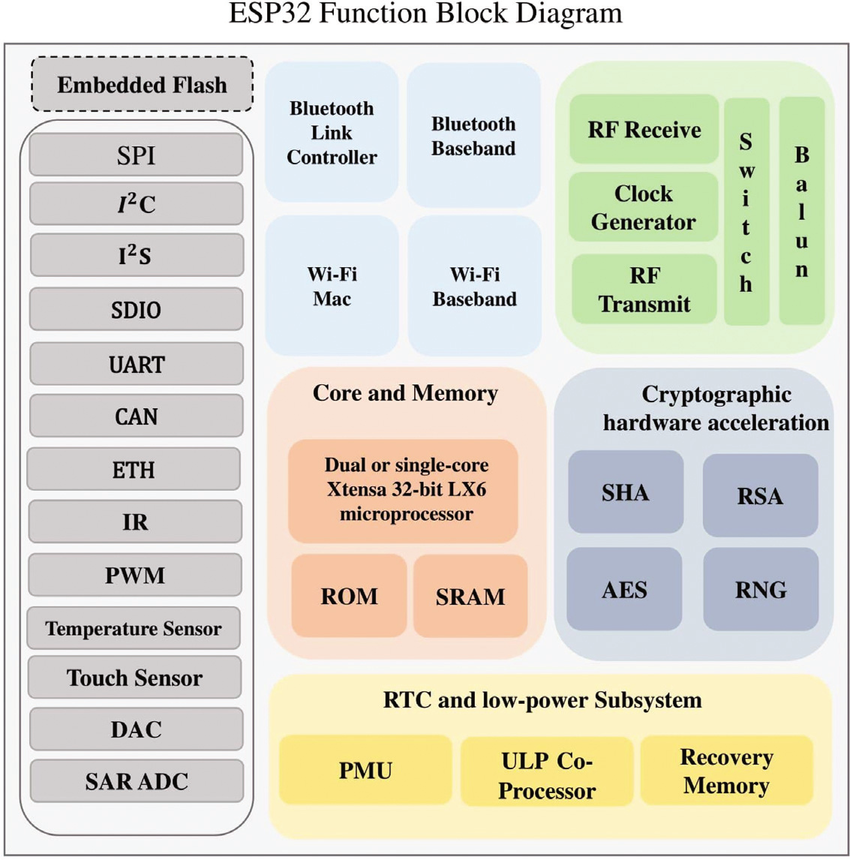
\includegraphics[width=0.9\textwidth]{esp32-block}
    \caption{Microcontrôleur ESP32}
    \label{fig:esp32}
\end{figure}

\subsection{Carte de développement ESP32-WROVER-B}
Le \textbf{microcontrôleur ESP32} est intégré dans une \textbf{carte de développement} basée sur le module \textbf{ESP32-WROVER-B}, fabriqué par \textbf{uPesy} (\textit{France}), sous la référence \textbf{ESP32 Wrover DevKit v2.1}. Cette carte présente plusieurs \textbf{avantages} :
\begin{itemize}
    \item \textbf{Brochage des principales entrées/sorties}, facilitant ainsi son utilisation pour le prototypage.
    \item \textbf{Alimentation et connexion USB-C} intégrées pour un usage simplifié.
    \item \textbf{Mémoire supplémentaire} pour des applications plus complexes.
    \item \textbf{Compatibilité breadboard}, idéale pour la réalisation de \textbf{prototypes}.
\end{itemize}


\section{Amplificateur opérationnel}\label{electronique:opamp}

Un \textbf{amplificateur opérationnel} est un dispositif électronique permettant 
d'amplifier une différence de tension. Il est également appelé \textit{Ampli OP}, 
\textit{AOP} ou \textit{ALI} (\textbf{Amplificateur Linéaire Intégré}). Il 
possède deux entrées, notées \(V_+\) et \(V_-\), ainsi qu'une sortie 
\(V_s\). La sortie de l'amplificateur opérationnel correspond au produit de 
la différence de tension entre les deux entrées, multiplié par un facteur, 
souvent très élevé.

C'est un \textbf{circuit actif}, ce qui signifie qu'il a besoin d'une 
alimentation externe pour fonctionner. Il nécessite à la fois une alimentation 
positive (\(V_{CC+}\)) et une alimentation négative (\(V_{CC-}\)). Dans 
certains cas, l'alimentation négative peut être fournie par la masse 
(\(V_{CC-} = \text{masse}\)).


\begin{minipage}{0.49\textwidth}
    \begin{figure}[H]
        \centering
        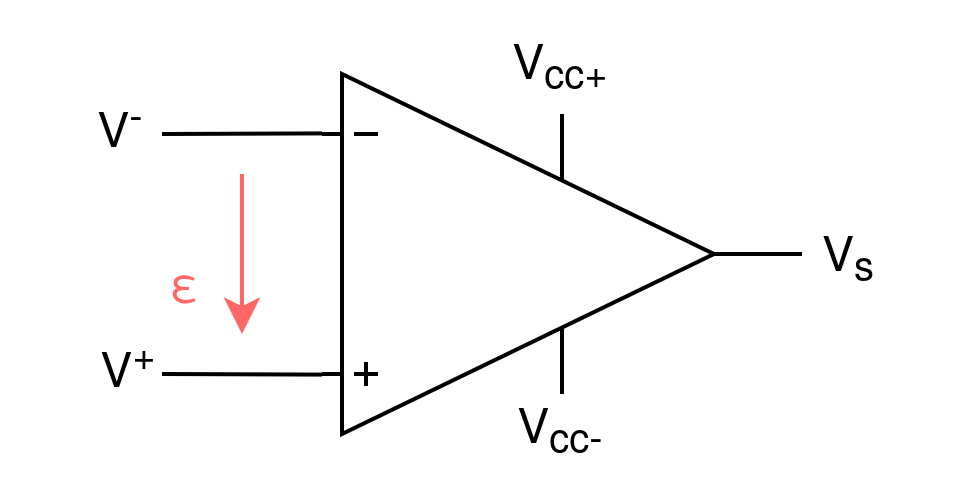
\includegraphics[width=0.9\textwidth]{opamp}
        \caption{Amplificateur opérationnel}
        \label{fig:opamp}
    \end{figure}
\end{minipage}
\begin{minipage}{0.5\textwidth}
    \begin{figure}[H]
        \centering
        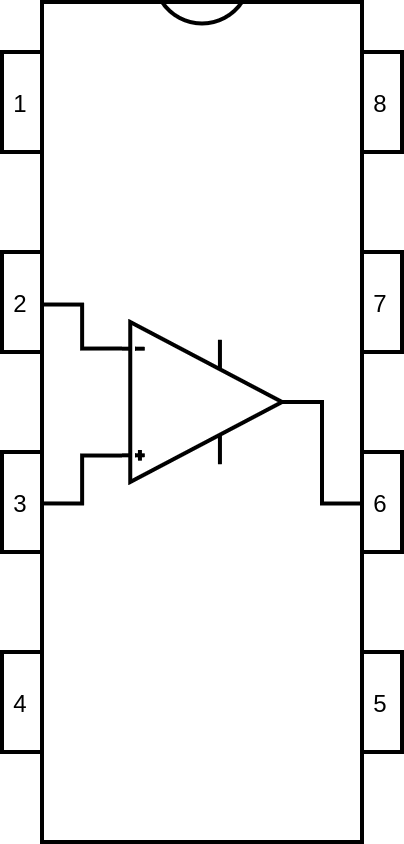
\includegraphics[width=0.3\textwidth]{MCP6271}
        \caption{Amplificateur opérationnel MCP6271}
        \label{fig:opamp-symbol}
    \end{figure}
\end{minipage}

L'entrée \(V_+\) est aussi appelée \textbf{entrée non inverseuse} (notée 
\(+\) sur le schéma), tandis que l'entrée \(V_-\) est appelée 
\textbf{entrée inverseuse} (notée \(-\) sur le schéma). L'alimentation 
positive \(V_{CC+}\) est parfois aussi désignée sous les appellations
\(V_{DD}\), \(V_{CC}\) ou \(V_{S+}\). De même, l'alimentation négative 
\(V_{CC-}\) peut être nommée \(V_{SS}\), \(V_{EE}\), \(V_{S-}\) ou 
encore \textbf{GND} si elle est connectée à la masse.

\section{Généralités sur les AOP}

L'alimentation électrique d'un \textbf{amplificateur opérationnel} (\textbf{AOP}
) peut être de deux types :
\begin{itemize}
    \item Une \textbf{alimentation simple} (\textit{single supply}), purement positive, par exemple \SI{0}{\volt} / \SI{+12}{\volt}.
    \item Une \textbf{alimentation symétrique} (\textit{dual supply}), où l'on dispose d'une tension négative et positive, par exemple \SI{-15}{\volt} / \SI{+15}{\volt}.
\end{itemize}

Certains AOP fonctionnent exclusivement avec une alimentation symétrique, 
d'autres uniquement avec une alimentation simple, et certains peuvent accepter 
les deux modes (\textit{cf. datasheet du composant}). Il est important de noter 
que l'alimentation conditionne directement le niveau de tension en sortie : un 
AOP alimenté en \SI{-12}{\volt} / \SI{+12}{\volt} ne pourra délivrer qu'une 
tension de sortie comprise entre \SI{-12}{\volt} et \SI{+12}{\volt}.

Un amplificateur opérationnel ne s'utilise quasiment jamais seul. En pratique, 
il est accompagné de composants électroniques additionnels tels que des 
\textbf{résistances}, des \textbf{condensateurs} et des \textbf{inductances}. 
Ces composants permettent d'utiliser l'AOP dans diverses applications :
\begin{itemize}
    \item \textbf{Calculs mathématiques analogiques} : addition, soustraction, inversion, intégration, dérivation, etc. Ces fonctions sont utilisées notamment pour le \textbf{pilotage et la régulation de moteurs électriques}.
    \item \textbf{Filtrage de signaux analogiques} : réalisation de filtres passe-bas, passe-haut, passe-bande, ou encore de filtres de rejet de bande. Ces filtres sont exploités dans des applications telles que le \textbf{filtrage audio}, le \textbf{mixage audio} ou encore l'atténuation de \textbf{bruits électroniques}.
    \item \textbf{Amplification de tensions et de courants} : un AOP peut être utilisé pour amplifier un signal avec adaptation d'impédance, ce qui est essentiel en \textbf{pré-amplification}, en \textbf{amplification} proprement dite, ainsi que pour la \textbf{régulation de tension et de courant}.
\end{itemize}

En interne un AOP est en fait un assemblage de plusieurs transistors, resistances et condensateurs. 
Il est donc possible de le modéliser par un schéma équivalent plus simple, 
appelé \textbf{schéma de représentation équivalent}.
\begin{figure}[H]
    \centering
    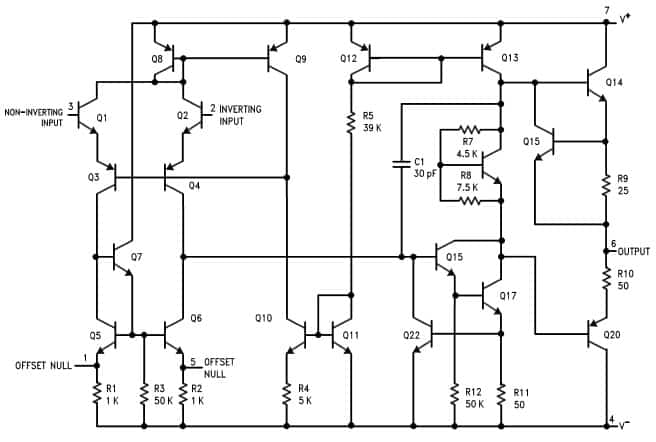
\includegraphics[width=0.9\textwidth]{LM741}
    \caption{
        Schéma équivalent d'un amplificateur opérationnel LM741
    }
    \label{fig:opamp-equivalent}
\end{figure}